% !TEX options=--shell-escape

\documentclass[a4paper,11pt,fleqn]{article}
%DIF LATEXDIFF DIFFERENCE FILE
%DIF DEL python-mip-tutorial.tex            Wed Nov 27 14:33:13 2019
%DIF ADD python-mip-tutorialSugestoes.tex   Wed Nov 27 16:21:10 2019
\usepackage{podes-template}

%pacotes adicionais
\usepackage[linesnumbered, algoruled, vlined, portuguese]{algorithm2e}
\usepackage{listings}
\usepackage{multirow}

%DIF 9a9-10
\usepackage{todonotes} %DIF > 
 %DIF > 
%DIF -------
\usepackage{colortbl}
\usepackage{xcolor}

\usepackage{minted}
% minted options
    \RequirePackage{minted}
    \AtBeginEnvironment{minted}{\let\itshape\relax}
    \AtBeginEnvironment{Verbatim}{\let\itshape\relax}
    \setminted{
        autogobble=true,
        baselinestretch=0.9,
        fontsize=\footnotesize,
        frame=single,
        framesep=3pt,
        linenos=true,
        mathescape=true,
        numbersep=8pt,
        tabsize=4,
        xleftmargin=15pt
    }
    \setmintedinline{
        linenos=false
    }

\lstset
{ %Formatting for code in appendix
    language=Python,
    numbers=left,
    stepnumber=1,
    showstringspaces=false,
    tabsize=1,
    breaklines=true,
    breakatwhitespace=false,
    extendedchars=true,
    literate={á}{{\'a}}1 {õ}{{\~o}}1 {ã}{{\~a}}1 {í}{{\'i}}1 {é}{{\'e}}1 {ç}{{\,c}}1,
}
%DIF 23a25
 %DIF > 
%DIF -------

\widowpenalty10000
\clubpenalty10000
\sloppy

%%%%%%%%%%%%%%%%%%%%%%%%%%%%%%%%%%% %%%%%%%%%%%%%%%%%%%%%%%%%%%%%%%%%%%%%%%


%título do artigo
\title{Tutorial de desenvolvimento de métodos de Programação Linear Inteira Mista em Python usando o pacote Python-MIP$^1$}

%define os autores
\author{
 \name{Haroldo G. Santos\authortag{a}\corresponding{haroldo@ufop.edu.br}}, 
 \name{T\'{u}lio A. M. Toffolo\authortag{a}} \\
 \authortag{a}
 \institute{Instituto de Ciências Exatas e Biológicas, Departamento de Computação\\ Universidade Federal de Ouro Preto, Ouro Preto, MG, Brasil}
}

\authorrunning{Santos \& Toffolo}
%DIF PREAMBLE EXTENSION ADDED BY LATEXDIFF
%DIF UNDERLINE PREAMBLE %DIF PREAMBLE
\RequirePackage[normalem]{ulem} %DIF PREAMBLE
\RequirePackage{color}\definecolor{RED}{rgb}{1,0,0}\definecolor{BLUE}{rgb}{0,0,1} %DIF PREAMBLE
\providecommand{\DIFadd}[1]{{\protect\color{blue}\uwave{#1}}} %DIF PREAMBLE
\providecommand{\DIFdel}[1]{{\protect\color{red}\sout{#1}}}                      %DIF PREAMBLE
%DIF SAFE PREAMBLE %DIF PREAMBLE
\providecommand{\DIFaddbegin}{} %DIF PREAMBLE
\providecommand{\DIFaddend}{} %DIF PREAMBLE
\providecommand{\DIFdelbegin}{} %DIF PREAMBLE
\providecommand{\DIFdelend}{} %DIF PREAMBLE
%DIF FLOATSAFE PREAMBLE %DIF PREAMBLE
\providecommand{\DIFaddFL}[1]{\DIFadd{#1}} %DIF PREAMBLE
\providecommand{\DIFdelFL}[1]{\DIFdel{#1}} %DIF PREAMBLE
\providecommand{\DIFaddbeginFL}{} %DIF PREAMBLE
\providecommand{\DIFaddendFL}{} %DIF PREAMBLE
\providecommand{\DIFdelbeginFL}{} %DIF PREAMBLE
\providecommand{\DIFdelendFL}{} %DIF PREAMBLE
%DIF LISTINGS PREAMBLE %DIF PREAMBLE
\lstdefinelanguage{codediff}{ %DIF PREAMBLE
  moredelim=**[is][\color{red}]{*!----}{----!*}, %DIF PREAMBLE
  moredelim=**[is][\color{blue}]{*!++++}{++++!*} %DIF PREAMBLE
} %DIF PREAMBLE
\lstdefinestyle{codediff}{ %DIF PREAMBLE
    belowcaptionskip=.25\baselineskip, %DIF PREAMBLE
    language=codediff, %DIF PREAMBLE
    basicstyle=\ttfamily, %DIF PREAMBLE
    columns=fullflexible, %DIF PREAMBLE
    keepspaces=true, %DIF PREAMBLE
} %DIF PREAMBLE
%DIF END PREAMBLE EXTENSION ADDED BY LATEXDIFF

\begin{document}


\maketitle

\begin{resumo}
O pacote Python-MIP oferece um conjunto abrangente de ferramentas para modelagem e resolução de Problemas de Programação Inteira Mista em Python. Além de oferecer uma linguagem de modelagem de alto nível, o pacote permite o desenvolvimento de métodos avançados, habilitando a comunicação bidirecional com o pacote de otimização durante o processo de busca. Neste tutorial, desenvolveremos métodos de Programação Linear Inteira Mista para o Problema do Caixeiro Viajante. Iniciando com um método simples baseado em uma formulação compacta iremos evoluir para um método que combina heurísticas e planos de corte para a resolução de problemas maiores.
\end{resumo}

\begin{palavras}
Otimização Combinatória, Caixeiro Viajante, Programação Linear Inteira, Python.
\end{palavras}

\begin{abstract}
The Python-MIP package offers a comprehensive set of tools for the modeling and solution of Integer Linear Programming Problems in Python. Besides providing a high level modeling language, the package allows the development of advanced solvers with bidirectional communication with the solver during the search process. In this tutorial we develop solvers for the Traveling Salesman Problem. Starting with a simple solver based on a compact formulation we evolve to a solver combining heuristics and cutting planes for the solution of larger instances.
\end{abstract}

\begin{keywords}
Combinatorial Optimization, Traveling Salesman Problem, Integer Linear \\Programming, Python. 
\end{keywords}


\newpage
\thispagestyle{defaultPage}

\section{Introdução}

Python-MIP é um software livre de código aberto\footnote{Mais informações em \url{www.python-mip.com}} para modelagem de Problemas de Programação Linear Inteira Mista \citep{Wolsey1998} em Python desenvolvido pelos autores deste tutorial.
O projeto do pacote foi concebido com o objetivo de desenvolver uma ferramenta que atenda aos seguintes requisitos:
\begin{enumerate}
	\item clareza de código e modelagem de alto nível;
	\item alto desempenho;
	\item extensibilidade e configurabilidade.
\end{enumerate}

Tradicionalmente, os requisitos 1 e 2 são considerados conflitantes.
Até recentemente, as opções mais recomendadas para os interessados no primeiro requisito eram linguagens algébricas de alto nível como AMPL \citep{Fourer1987}.
A obtenção de desempenho máximo costumava requerer o uso de linguagens de mais baixo nível como C \citep{Johnson1991a}. 
Pacotes de otimização estado-da-arte como o CPLEX foram escritos nessa linguagem \citep{Bixby2002}. 
Desse modo, a biblioteca completa de funções estava originalmente disponível somente nela. 
Recentemente, soluções como JuMP \citep{Dunning2015,Castellucci2017} demonstraram que os requistos 1 e 2 não são necessariamente conflitantes: linguagens de alto nível como Julia juntamente com compiladores \emph{just-in-time} permitem o desenvolvimento rápido de métodos que apresentam alto desempenho. 
O objetivo do projeto Python-MIP é o desenvolvimento de um pacote de modelagem e desenvolvimento de algoritmos de Programação Linear Inteira Mista para a linguagem Python que atenda plenamente aos três requisitos destacados anteriormente.

Pesquisas recentes mostram que Python está se tornando a linguagem mais popular da atualidade \citep{pythonEconomist2018}. 
O projeto Python-MIP foi inspirado em dois projetos de código aberto para programação linear inteira em Python. 
O primeiro é o PuLP \citep{Mitchell2009}, que oferece uma linguagem de modelagem de alto nível e interface para vários pacotes de otimização comerciais e de código aberto. 
No entanto, recursos que requerem uma integração maior com o pacote, como geração dinâmica de planos de cortes, não estão disponíveis neste pacote. 
O pacote CyLP, por outro lado, suporta geração dinâmica de planos de corte mas não oferece uma linguagem de modelagem de alto nível \citep{Towhidi2016}, mas é compatível apenas com o pacote de otimização COIN-OR CBC \citep{Forrest2005}. 
O pacote Python-MIP foi criado com o objetivo de prover a funcionalidade dos dois pacotes com máximo desempenho. 
A escrita de um um novo pacote de programação linear inteira em Python também permite que recursos relativamente novos da linguagem, como a tipagem estática e a comunicação direta com bibliotecas nativas (Python CFFI) sejam utilizados extensivamente no código.

Neste tutorial, apresentaremos versões sucessivamente mais sofisticadas de um método para resolver o clássico Problema do Caixeiro Viajante \citep{Dantzig54,Miller1960,Applegate2006}, que é brevemente descrito na Seção \ref{secTSP}.
Os métodos foram desenvolvidos utilizando o pacote Python-MIP. 
Enquanto na primeira versão a comunicação com o pacote de otimização ocorre somente nos momentos de criação do modelo e coleta dos resultados, a versão final utiliza comunicação bidirecional com o pacote de otimização durante o processo de busca para o tratamento de uma formulação com um número exponencial de restrições em um método \emph{branch\&cut}. 
Resultados experimentais são apresentados na Seção \ref{secExp} para demonstrar os ganhos substanciais de desempenho que podem ser obtidos com essa última versão.

\section{Aplicação: Problema do Caixeiro Viajante}
\label{secTSP}

O problema do caixeiro viajante consiste em: dada uma malha viária e um conjunto de pontos que devem ser visitados, encontrar uma rota de custo mínimo (tempo ou distância, usualmente) que inclua todos os pontos percorrendo-os exatamente uma vez. 
Formalmente, temos como dados de entrada um grafo direcionado $G=(V,A)$ com custos associadas aos arcos:
\begin{description}
	\item [{$V$}] é o conjunto de vértices, $V=\{0,1,...,n\}$;
    % \item [{$A$}] é o conjunto de arcos que conectam os vértices em $V$, $A = V \times V$;
	\item [{$c_{i,j}$}] é custo de percorrer a arco $(i, j) \in A$
\end{description}

Em todas as formulações consideradas neste tutorial, utilizamos as seguintes variáveis binárias de decisão que representam a escolha dos arcos que compõem a rota:
\[
x_{i,j}=\begin{cases}
1 & \textrm{se o arco }(i,j)\textrm{ foi escolhido para a rota}\\
0 & \textrm{caso contrário}
\end{cases}
\]
Como exemplo, considere o mapa da Figura \ref{figG} que inclui quatorze cidades turísticas da Bélgica.

\begin{figure}
	\begin{centering}
		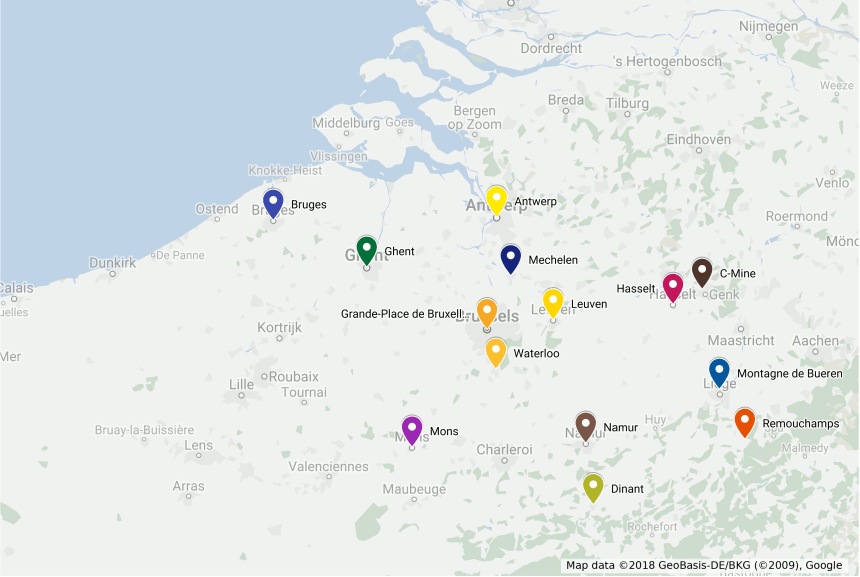
\includegraphics[width=0.6\textwidth]{../images/belgium-tourism-14.png}
		\par\end{centering}
	\caption{14 cidades turísticas da Bélgica}	
	\label{figG}
\end{figure}


\subsection{Uma Formulação Compacta}

O problema do caixeiro viajante pode ser modelado utilizando-se uma formulação compacta, isto é, uma formulação com um número polinomial de variáveis e de restrições. 
Formulações desse tipo, apesar de usualmente não serem a melhor opção de resolução em termos de desempenho para o problema, são convenientes para uma primeira abordagem pois podem ser facilmente inseridas de uma vez só como entrada para um pacote de otimização. 
A formulação \eqref{m1fo}-\eqref{m1bin} foi proposta por \cite{Miller1960}:
\allowdisplaybreaks
\begin{align}
    \label{m1fo} \textrm{Minimize: }   & \nonumber \\
    &  \sum_{i \in V} \sum_{j \in V} c_{i,j} \ldotp x_{i,j} \\
    \textrm{Sujeito a: }   & \nonumber \\
    & \sum_{j \in V \setminus \{i\}} x_{i,j} = 1 \,\,\, \forall i \in V \label{eq:in}  \\
    & \sum_{i \in V \setminus \{j\}} x_{i,j} = 1 \,\,\, \forall j \in V \label{eq:out} \\
    & y_{i} -(n+1)\ldotp x_{i,j} \geq y_{j} -n  \,\,\, \forall i \in V\setminus \{0\}, j \in V\setminus \{0,i\} \label{eq:st1} \\
    & x_{i,j} \in \{0,1\} \,\,\, \forall i \in V, j \in V \\
    \label{m1bin} & y_i \geq 0 \,\,\, \forall i \in V 
\end{align}

A função objetivo (\ref{m1fo}) minimiza o custo total da rota. As equações (\ref{eq:in}) e (\ref{eq:out}), denominadas restrições de grau, garantem que cada vértice é visitado somente uma vez enquanto variáveis auxiliares $y_{i}$ são utilizadas nas restrições (\ref{eq:st1}) para garantir que uma vez que um arco $(i,j)$ seja selecionado, o valor de $y_{j}$ seja maior do que o valor de $y_{i}$ em uma unidade. 
Essa propriedade é garantida para todos os vértices exceto o vértice 0, que é arbitrariamente selecionado como origem de modo a evitar a construção de sub-rotas desconectadas, como no exemplo da Figura \ref{figSub}, onde os valores das variáveis $x_{i,j}$ indicados nos arcos representam uma solução viável se somente as restrições (\ref{eq:in}) e (\ref{eq:out}) fossem consideradas.

\begin{figure}[h!]
	\begin{centering}
		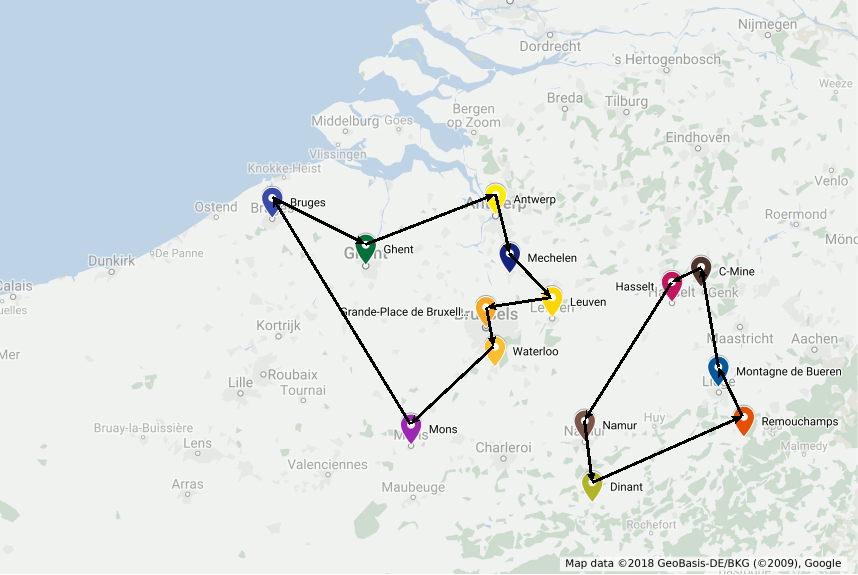
\includegraphics[width=0.6\textwidth]{belgium-tourism-14-subtour.png}
		\par\end{centering}
	\caption{Rotas desconectadas da origem}
	\label{figSub}
\end{figure}

\subsection{Implementação do modelo usando o Python-MIP}

Destacamos que a instalação do pacote é bastante simples. 
Recomenda-se fazer a instalação por meio do instalador de pacotes pip\footnote{O pip está disponível gratuitamente em \url{pypi.org/project/pip}}.
% Depois da instalação da linguagem Python e o gerenciador de pacotes da mesma (pip) pode ser invocado para instalação. 
Utilizando o pip, para instalar o Python-MIP basta executar o seguinte comando no terminal do sistema:

\begin{minted}[linenos=false]{bash}
    pip install mip --user
\end{minted}

A seguir temos um exemplo completo de um modelo escrito em Python-MIP para resolver o Problema do Caixeiro Viajante para o mapa da Figura \ref{figG}.
O código a seguir utiliza a formulação compacta dada pelas equações \eqref{m1fo}-\eqref{m1bin}, descrita anteriormente:

\begin{minted}{python}
    from itertools import product
    from sys import stdout as out
    from mip import Model, xsum, minimize, BINARY

    # lugares de visitação
    places = ['Antwerp', 'Bruges', 'C-Mine', 'Dinant', 'Ghent',
              'Grand-Place de Bruxelles', 'Hasselt', 'Leuven',
              'Mechelen', 'Mons', 'Montagne de Bueren', 'Namur',
              'Remouchamps', 'Waterloo']

    # distâncias em matriz triangular superior
    dists = [[83, 81, 113, 52, 42, 73, 44, 23, 91, 105, 90, 124, 57],
             [161, 160, 39, 89, 151, 110, 90, 99, 177, 143, 193, 100],
             [90, 125, 82, 13, 57, 71, 123, 38, 72, 59, 82],
             [123, 77, 81, 71, 91, 72, 64, 24, 62, 63],
             [51, 114, 72, 54, 69, 139, 105, 155, 62],
             [70, 25, 22, 52, 90, 56, 105, 16],
             [45, 61, 111, 36, 61, 57, 70],
             [23, 71, 67, 48, 85, 29],
             [74, 89, 69, 107, 36],
             [117, 65, 125, 43],
             [54, 22, 84],
             [60, 44],
             [97],
             []]

    # número de nós e lista de vértices
    n, V = len(dists), set(range(len(dists)))

    # matriz de distâncias completa
    c = [[0 if i == j
          else dists[i][j-i-1] if j > i
          else dists[j][i-j-1]
          for j in V] for i in V]

    model = Model()

    # variáveis binárias indicando se arco (i,j) é usado na rota
    x = [[model.add_var(var_type=BINARY) for j in V] for i in V]

    # variáveis contínuas para prevenção de sub-rotas: cada cidade terá
    # um identificador numérico maior na rota, excetuando-se a primeira
    y = [model.add_var() for i in V]

    # função objetivo: minimizar custo total
    model.objective = minimize(xsum(c[i][j]*x[i][j] for i in V for j in V))

    # restrição : sair de cada cidade somente uma vez
    for i in V:
        model += xsum(x[i][j] for j in V - {i}) == 1

    # restrição : entrar em cada cidade somente uma vez
    for i in V:
        model += xsum(x[j][i] for j in V - {i}) == 1

    # eliminação de sub-rotas
    for (i, j) in product(V - {0}, V - {0}):
        if i != j:
            model += y[i] - (n+1)*x[i][j] >= y[j]-n

    # otimização com limite de tempo de 30 segundos
    model.optimize(max_seconds=30)

    # verificando se ao menos uma solução válida foi encontrada
    if model.num_solutions:
        out.write('route with total distance %g found: %s'
                  % (model.objective_value, places[0]))
        nc = 0
        while True:
            nc = [i for i in V if x[nc][i].x >= 0.99][0]
            out.write(' -> %s' % places[nc])
            if nc == 0:
                break
        out.write('\n')
\end{minted}

Nas linhas 6-9 nomeamos nossos pontos turísticos. 
Nas linhas 12-25 informamos o tempo estimado de deslocamento entre cada par de cidades $(i, j)$ onde $i<j$, visto que para nosso exemplo consideramos que as distâncias de ida e volta são iguais, ou seja, temos um Problema do Caixeiro Viajante Simétrico. 
Convertemos a matriz triangular \texttt{dists} em uma matriz completa nas linhas 31-34.

A linha 36 cria um modelo de programação linear inteira. 
As variáveis do modelo são criadas nas linhas 39 e 43 utilizando o método \texttt{add\_var} em nosso modelo \texttt{model}. 
Durante a criação das restrições, é necessário referenciar as variáveis criadas. 
Por isso, utilizamos a matriz \texttt{x} para mapear cada arco do grafo com sua respectiva variável binária.
% Destacamos que, se um grafo esparso fosse informado poderíamos utilizar um vetor de dicionários para indicar os arcos de saída de cada nó. 
O vetor \texttt{y} é utilizado para mapear cada nó com sua respectiva variável auxiliar contínua para eliminação de sub-rotas.

A função objetivo que minimiza o tempo total gasto para percorrer a rota é informada na linha 46. 
Nesse caso, para cada arco multiplicamos sua respectiva variável binária de seleção pelo tempo de deslocamento do arco armazenado em \texttt{c}.

As restrições são criadas nas linhas 48-59. Em todos os casos utilizamos o operador \texttt{+=} sobre o modelo \texttt{m} para adicionar restrições lineares. Note que assim como na função objetivo, o somatório é efetuado com a função \texttt{xsum}. Esta função é similar a função \texttt{sum} disponível na linguagem Python mas otimizada para a situação específica de escrita de restrições lineares no pacote Python-MIP\@. 

A linha 62 dispara a otimização do modelo indicando um limite de tempo para a otimização de 30 segundos. Na linha 65 verificamos se uma solução viável foi encontrada e, em caso positivo, a escrevemos nas linhas 65-74.

Os pacotes de programação linear inteira executam uma busca em árvore onde são utilizados \emph{limites} para a poda de nós. O limite superior é obtido a partir de qualquer solução viável que for encontrada durante a busca e o limite inferior corresponde ao custo obtido com a resolução do problema com as restrições de integralidade das variáveis relaxadas. No nosso caso considerando domínio das variáveis $x$ como contínuo entre 0 e 1. A formulação aqui utilizada tem uma grave deficiência: o limite inferior por ela produzido é distante do custo ótimo da solução. Desse modo, o desempenho dos pacotes de programação linear inteira em sua resolução é bastante pobre. Essa deficiência não é visível quando resolvemos problemas pequenos como o de exemplo (apenas 14 cidades), mas faz com que o desempenho do pacote degenere muito rapidamente a medida que o tamanho do grafo de entrada aumenta. Na seção seguinte veremos o tratamento de uma formulação mais apropriada.

\subsection{Formulações Fortes com Geração Dinâmica de Restrições}

A formulação do caixeiro viajante utilizada nos métodos de melhor desempenho inclui restrições de eliminação de sub-rotas do tipo:

\begin{equation}
	\sum_{(i,j) \in S \times S} x_{(i,j)} \leq |S|-1 \,\,\, \forall S \subset V \label{consSubTour}
\end{equation}

O problema das desigualdades acima é que elas devem ser geradas para \emph{cada subconjunto} $S$ de vértices do grafo, ou seja, para um grafo com $n$ vértices temos $2^n-1$ subconjuntos não vazios. 
Inseri-las no modelo inicial é inviável, exceto para instâncias pequenas. 
Uma solução para esse problema é inserir somente as restrições \emph{necessárias} no modelo, com o método dos Planos de Corte \citep{Dantzig54}. 
O pacote Python-MIP permite uma comunicação bi-direcional com o resolvedor para que as restrições necessárias sejam inseridas \emph{durante} a busca. 
Para isso precisamos criar uma classe derivada da classe \texttt{ConstrsGenerator} que implemente o método \texttt{generate\_constrs}. 
Esse método recebe como parâmetro um modelo, onde a solução corrente pode ser consultada e restrições adicionais podem ser inseridas na medida do necessário, caso a solução corrente não as satisfaça. 

O pacote Python-MIP permite um controle sobre em que ponto da busca as restrições faltantes são verificadas. 
Duas propriedades do modelo podem ser preenchidas com objeto(s) do tipo \texttt{ConstrsGenerator}:

\begin{description}
	\item[\texttt{cuts\_generator}]: caso o gerador de restrições seja informado com essa propriedade do modelo, a verificação por restrições faltantes (cortes violados) é realizada sempre que uma \emph{solução fracionária} for gerada durante a resolução de um nó na árvore de busca. Nesse caso, cortes são inseridos para \emph{reforçar} a formulação inserida inicialmente, ou seja, caso somente um \texttt{cuts\_generator} seja informado é necessário que a formulação inicial seja completa; assim, caso a restrição (\ref{consSubTour}) seja inserida dessa forma, as variáveis auxiliares $y$ e as restrições (fracas) de eliminação de sub-ciclos devem ser mantidas na formulação inicial visto que as restrições de grau não são suficientes para definir uma solução factível.
	
	\item[\texttt{lazy\_constrs\_generator}]: um gerador de restrições informado com essa propriedade é chamado sempre que uma \emph{solução inteira} for gerada. Nesse modo de uso é possível iniciar a busca com uma formulação incompleta, ou seja, sem as variáveis auxiliares $y$ e as restrições (4). Desse modo, a formulação inicial pode ficar muito mais leve. Uma possível desvantagem dessa abordagem é que como o pacote de otimização deve considerar que a formulação inicial está \emph{incompleta}, algumas fases do pré-processamento do mesmo precisam ser desligadas e o limite inferior inicial pode ser menor.
\end{description}

Assim, uma vez que tenhamos um gerador de restrições implementado (especialização da classe \texttt{ConstrsGenerator}), podemos decidir em que situação o mesmo será chamado. É possível também especificar geradores de restrições para ambas as situações, ou seja, a formulação inicial é incompleta e portanto toda solução inteira deve ser checada mas soluções fracionárias também são verificadas. A melhor abordagem a ser utilizada deve ser determinada com experimentos para o problema de interesse. 
Na Seção \ref{secExp} são incluídos experimentos para diferentes configurações do nosso código.

O código a seguir implementa um gerador dinâmico de restrições de eliminação de sub-rotas em soluções inteiras para nossa formulação compacta previamente implementada. 

\begin{minted}{python}
    from mip.callbacks import ConstrsGenerator, CutPool
    from typing import Set, List
    from collections import defaultdict

    def subtour(N: Set, outa: defaultdict, node) -> List:
        """verifica se 'node' pertence a alguma sub-rota e retorna os 
        nós envolvidos"""
        queue = [node]
        visited = set(queue)
        while queue:
            n = queue.pop()
            for nl in outa[n]:
                if nl not in visited:
                    queue.append(nl)
                    visited.add(nl)

        if len(visited) != len(N):
            return [v for v in visited]
        else:
            return []

    class SubTourLazyGenerator(ConstrsGenerator):
        def __init__(self, xv):
            self._x = xv

        def generate_constrs(self, model: Model):
            """restrições de eliminação de sub-rotas em soluções inteiras"""
            x_, N = model.translate(self._x), range(len(self._x))
            cp = CutPool()
            outa = [[j for j in N if x_[i][j].x >= 0.99] for i in N]

            for node in N:
                S = set(subtour(N, outa, node))
                if S:
                    AS = [(i, j) for (i, j) in product(S, S) if i != j]
                    cut = xsum(x_[i][j] for (i, j) in AS) <= len(S)-1
                    cp.add(cut)
            for cut in cp.cuts:
                model += cut
\end{minted}

Em soluções inteiras como a da Figura 2, a identificação de sub-rotas pode ser facilmente realizada executando-se uma busca em profundidade a partir de cada nó e verificando sua conectividade (função \texttt{subtour}). Na função de geração de restrições, as referências para as variáveis x originais do modelo são atualizadas para o modelo corrente com o método \texttt{translate} (linha 28). A existência ou não de um arco depende do valor da respectiva variável $x$ na solução inteira. O arco de saída associado com cada nó é computado na linha 30. Para cada nó, caso uma sub-rota desconectada seja identificada (linha 33) uma restrição do tipo (\ref{consSubTour}) é gerada para o subconjunto \texttt{S} envolvido. Os cortes são temporariamente armazenados em um objeto do tipo \texttt{CutPool} pois o mesmo descarta cortes repetidos. Finalmente, nas linhas 38-39, os cortes são adicionados ao modelo.


Para que esse código seja executado durante a busca, antes de chamar a otimização do modelo no código anterior (linha 60), precisamos informar o gerador atribuindo um objeto desse tipo à propriedade \texttt{lazy\_constrs\_generator} com o código. Passamos como parâmetro do construtor de nosso gerador de restrições a matriz de variáveis x, que será consultada para verificação de conectividade: 

\begin{minted}[linenos=false]{python}
    model.lazy_constrs_generator = SubTourLazyGenerator(x)
\end{minted}

A versão completa do código que inclui a geração dinâmica de restrições de eliminação de sub-rotas em soluções inteiras pode ser obtida no repositório do Python-MIP\footnote{Exemplo \texttt{tsp-lazy.py}, disponível no repositório Python-MIP em \url{www.python-mip.com}}.

A geração de desigualdades que eliminam \emph{soluções fracionárias} determina o problema conhecido como \emph{separação de cortes}. No nosso caso queremos encontrar sub-conjuntos de vértices pouco conectados (não necessariamente desconectados) do restante da rota. Esse problema pode ser resolvido solucionando-se o problema do \emph{corte mínimo} considerando o grafo da malha viária do problema com o valor das variáveis $x$ como capacidades nos arcos. 
Para nosso exemplo, utilizaremos a implementação do algoritmo de corte mínimo disponível no pacote Python \texttt{networkx} para resolver esse problema.

\begin{minted}{python}
    import networkx as nx

    class SubTourCutGenerator(ConstrsGenerator):
        def __init__(self, Fl: List[Tuple[int, int]], x_, V_):
            self.F, self.x, self.V = Fl, x_, V_

        def generate_constrs(self, model: Model):
            xf, V_, cp = model.translate(self.x), self.V, CutPool()
            for (u, v) in [(k, l) for (k, l) 
                           in product(V_, V_) if k != l and xf[k][l]]:
                G.add_edge(u, v, capacity=xf[u][v].x)
            for (u, v) in F:
                val, (S, NS) = nx.minimum_cut(G, u, v)
                if val <= 0.99:
                    aInS = [(xf[i][j], xf[i][j].x)
                            for (i, j) in product(V_, V_) 
                            if i != j and xf[i][j] and i in S and j in S]
                    if sum(f for v, f in aInS) >= (len(S)-1)+1e-4:
                        cut = xsum(1.0*v for v, fm in aInS) <= len(S)-1
                        cp.add(cut)
                        if len(cp.cuts) > 256:
                            for cut in cp.cuts:
                                model += cut
                            return
            for cut in cp.cuts:
                model += cut

\end{minted}

Na criação de nosso gerador de cortes informamos uma lista \texttt{Fl} de pares $(i,j)$ de vértices cuja conectividade deve ser verificada em toda solução gerada. A descoberta de sub-rotas desconexas é feita nas linhas 13-14. Na linha 21 inserimos um critério de parada para a geração dos cortes: caso um número suficientemente grande já tenha sido gerado, inserimos os mesmos no modelo e prosseguimos a otimização sem procurar por cortes adicionais. Nesse ponto convém ressaltar a função dos cortes e sua relação com o restante do modelo. Como a formulação compacta que estamos utilizando define completamente o problema, a adição de cortes é opcional, ou seja, somente feita para melhorar o desempenho do modelo. A inserção de um número muito grande de cortes por iteração pode gerar o efeito indesejado de perda de desempenho na resolução. Para utilizarmos nosso gerador de cortes com a formulação anterior basta atribuir à propriedade \texttt{cuts\_generator} um objeto da nossa classe \texttt{SubTourCutGenerator} antes da otimização do modelo. O exemplo completo está disponível no repositório Python-MIP\footnote{Exemplo \texttt{tsp-cuts.py}, disponível no repositório Python-MIP em \url{www.python-mip.com}}.

\subsection{Integração com heurísticas}

Pacotes de programação linear inteira iniciam o processo de resolução computando uma solução possivelmente fracionária, obtida através da relaxação do problema. Em instâncias difíceis, a obtenção da primeira solução \emph{inteira} válida pode requerer a exploração de um grande número de nós na árvore de busca. Para essas instâncias, muitas vezes uma heurística simples e rápida pode ser utilizada para geração de uma solução inicial. No pacote Python-MIP, soluções iniciais podem ser facilmente informadas ao pacote de otimização através da propriedade \texttt{start} do modelo que recebe uma lista de pares \texttt{(x, v)} onde \texttt{x} é uma referência para uma variável de decisão e \texttt{v} o seu valor na solução factível. 

O código abaixo exemplifica a utilização de um algoritmo construtivo e de uma meta-heurística de busca local para construção de uma solução inicial factível para o problema considerado.
 
\begin{minted}{python}
    seq = [0, max((c[0][j], j) for j in V)[1]] + [0]
    Vout = V-set(seq)
    while Vout:
        (j, p) = min([(c[seq[p]][j] + c[j][seq[p+1]], (j, p)) for j, p in
                      product(Vout, range(len(seq)-1))])[1]

        seq = seq[:p+1]+[j]+seq[p+1:]    
        Vout = Vout - {j}


    def delta(d: List[List[float]], S: List[int], p1: int, p2: int) -> float:
        p1, p2 = min(p1, p2), max(p1, p2)
        e1, e2 = S[p1], S[p2]
        if p1 == p2:
            return 0
        elif abs(p1-p2) == 1:
            return ((d[S[p1-1]][e2] + d[e2][e1] + d[e1][S[p2+1]])
                    - (d[S[p1-1]][e1] + d[e1][e2] + d[e2][S[p2+1]]))
        else:
            return ((d[S[p1-1]][e2] + d[e2][S[p1+1]] + 
                     d[S[p2-1]][e1] + d[e1][S[p2+1]])
                  - (d[S[p1-1]][e1] + d[e1][S[p1+1]] + 
                     d[S[p2-1]][e2] + d[e2][S[p2+1]]))

    L = [cost for i in range(50)]
    sl, cur_cost, best = seq.copy(), cost, cost
    for it in range(int(1e7)):
        (i, j) = rnd.randint(1, len(sl)-2), rnd.randint(1, len(sl)-2)
        dlt = delta(c, sl, i, j)
        if cur_cost + dlt <= L[it % len(L)]:
            sl[i], sl[j], cur_cost = sl[j], sl[i], cur_cost + dlt
            if cur_cost < best:
                seq, best = sl.copy(), cur_cost
        L[it % len(L)] = cur_cost
        
    m.start = [(x[seq[i]][seq[i+1]], 1) for i in range(len(seq)-1)]    
\end{minted}

Nosso algoritmo construtivo (linhas 3-8) é o algoritmo da inserção mais barata: iniciamos uma rota parcial incluindo arbitrariamente as ligações $(0, j)$ e $(j, 0)$ (linha 6), onde $j$ é o ponto mais distante do ponto inicial e prosseguimos aumentando a rota. Na inserção de um novo ponto verificamos o custo de inserir \emph{cada vértice} ainda fora da rota (conjunto \texttt{Vout} em \emph{cada posição} intermediária possível (\texttt{p}) e selecionamos a opção mais barata. A inserção de um novo ponto utiliza os recursos de fatiamento e adição de listas da linguagem Python (linha 7).

Para melhoria da solução inicial, utilizamos a meta-heurística baseada em busca local Late Acceptance Hill Climbing \citep{burke2017} por sua simplicidade. O gargalo de métodos de busca local usualmente é a avaliação do custo da solução resultante da aplicação de dado movimento. Por isso, nas linhas 11-22 incluímos uma função que dada uma solução de entrada (sequência de cidades) \texttt{s} e duas posições dessa sequência, \texttt{p1} e \texttt{p2} calcula em \emph{tempo constante} a variação de custo que será obtida. Dessa forma, podemos executar rapidamente um grande número de movimentos cuja aceitação é controlada pelo arcabouço da meta-heurística que é implementada nas linhas 25-33. Finalmente, informamos as variáveis de decisão relacionadas aos arcos existentes na melhor solução encontrada na linha 35.

\section{Experimentos Computacionais} \label{secExp}

Para analisar a melhoria de desempenho que pode ser obtida com a geração
dinâmica de restrições e com a integração com heurísticas, incluímos neste tutorial experimentos com diferentes versões de nosso método:

\begin{description}
	\item[\textsc{MTZ}]: método que utiliza a formulação compacta somente;
	\item[\textsc{MTZ+H}]: método que utiliza a formulação compacta e a heurística para produção de uma solução inicial factível;
	\item[\textsc{MTZ+C}]: método que utiliza a formulação compacta e a geração dinâmica de restrições para eliminação de soluções fracionárias (planos de corte);
	\item[\textsc{LAZY}]: método em que somente as restrições de grau (2) e (3) são inicialmente informadas, enquanto as restrições de eliminação de sub-rotas são inseridas por demanda;
	\item[\textsc{LAZY+C+H}]: método em que somente as restrições de grau (2) e (3) são inicialmente informadas, enquanto as restrições de eliminação de sub-rotas e planos de corte são inseridas por demanda e uma solução inicial inteira é informada.
\end{description}

Os testes utilizaram a versão 1.5.3 do pacote Python-MIP. Foram avaliados como motor de busca ou o pacote de otimização COIN-OR CBC, incluso no pacote, ou o pacote comercial Gurobi 8.1\footnote{\url{www.gurobi.com}}. 
Uma das vantagens do pacote Python-MIP é que nenhuma linha de código precisa ser modificada caso o usuário queira trocar de motor de busca: todas as funcionalidades são compatíveis com ambos os motores. 
Os experimentos foram executados em um computador com processador Intel Core i7-4960X 3.6 GHz com 32 Gb de RAM. 
Cada teste foi realizado de maneira sequencial, sendo que o pacote GNU Parallel \citep{Tange2011} foi empregado para que os núcleos fossem utilizados em paralelo, executando diferentes testes. 
Um tempo limite de dez horas (36.000 segundos) foi estipulado para cada execução. 
Algumas instâncias com até 202 nós da coleção de problemas TSPLIB95 \citep{Reinelt95} foram selecionadas. 
Os resultados (tempos de execução em segundos) são apresentados na Tabela \ref{resExp}. O sufixo numérico no nome das instâncias indica o número de pontos que cada uma inclui. O melhor resultado para cada instância é enfatizado em negrito. Células com execuções que foram truncadas por tempo foram sombreadas.
    
Como podemos observar, instâncias com algumas centenas de nós são claramente difíceis de resolver utilizando a formulação fraca MTZ, independente do pacote de otimização utilizado. A adição por demanda de restrições de eliminação de sub-rotas (versões com +C e/ou LAZY) oferece ganhos expressivos, de modo similar para os dois pacotes de otimização. A aceleração média obtida para o CBC foi de mais de 80 vezes e para o Gurobi de mais de 60 vezes. Esse número é uma estimativa baixa da aceleração obtida, pois as execuções foram truncadas por tempo. Esses resultados ilustram a importância do estudo e implementação computacional de diferentes formulações para o tratamento de um problema de otimização combinatória. Leitores interessados no estado-da-arte em métodos de resolução para o problema do caixeiro viajante podem consultar o texto de \cite{Cook2019}.

\begin{table}
	\begin{center}		
    \caption{Resultados de experimentos computacionais para os métodos desenvolvidos utilizando os pacotes de otimização CBC e Gurobi\vspace{10pt}}
    \label{resExp}
\begin{tabular}{|r|r|r|r|r|r|}
\hline 
\multirow{2}{*}{instância} & \multicolumn{5}{c|}{Python-MIP 1.5.3 com CBC}\tabularnewline
\cline{2-6} \cline{3-6} \cline{4-6} \cline{5-6} \cline{6-6} 
 & \textsc{mtz} & \textsc{mtz+h} & \textsc{mtz+c} & \textsc{lazy} & \textsc{lazy+c+h}\tabularnewline
\hline 
\hline 
ulysses22 & 778,0 & 1.292,5 & 7,4 & \cellcolor{gray}36.000,0 & 3,3\tabularnewline
\hline 
att48 & 13.578,6 & 12.749,2 & 14,8 & 14.546,7 & \textbf{5,9}\tabularnewline
\hline 
bier127 & \cellcolor{gray}36.000,0 & \cellcolor{gray}36.000,0 & 2.637,6 & \cellcolor{gray}36.000,0 & 136,3\tabularnewline
\hline 
gr202 & \cellcolor{gray}36.000,0 & \cellcolor{gray}36.000,0 & 2.613,0 & \cellcolor{gray}36.000,0 & \textbf{867,9}\tabularnewline
\hline 
\hline 
\emph{média} & 17.271,3 & 17.208,3 & 1.054,6 & 24.509,3 & \textbf{202,7}\tabularnewline
\hline 
\multicolumn{1}{r}{} & \multicolumn{1}{r}{} & \multicolumn{1}{r}{} & \multicolumn{1}{r}{} & \multicolumn{1}{r}{} & \multicolumn{1}{r}{}\tabularnewline
\hline 
\multirow{2}{*}{instância} & \multicolumn{5}{c|}{Python-MIP 1.5.3 com GUROBI}\tabularnewline
\cline{2-6} \cline{3-6} \cline{4-6} \cline{5-6} \cline{6-6} 
 & \textsc{mtz} & \textsc{mtz+h} & \textsc{mtz+c} & \textsc{lazy} & \textsc{lazy+c+h}\tabularnewline
\hline 
\hline 
ulysses22 & 148,1 & 214,1 & \textbf{1,7} & 66,5 & 3,1\tabularnewline
\hline 
att48 & 186,5 & 185,7 & 6,5 & 257,7 & 6,4\tabularnewline
\hline 
bier127 & \cellcolor{gray}36.000,0 & 25.508,8 & 209,3 & 884,0 & \textbf{79,7}\tabularnewline
\hline 
gr202 & \cellcolor{gray}36.000,0 & \cellcolor{gray}36.000,0 & 1.057,2 & 36.000,0 & 1.084,8\tabularnewline
\hline 
\hline 
\emph{média} & 14.466,9 & 12.381,7 & 254,9 & 7.441,6 & 234,8\tabularnewline
\hline 
\end{tabular}
	\end{center}	
\end{table}

\section{Conclusões}

Neste tutorial foram desenvolvidos e avaliados computacionalmente diferentes métodos exatos para o clássico Problema do Caixeiro Viajante utilizando o pacote Python-MIP. 
Experimentos computacionais foram realizados demonstrando os ganhos expressivos que podem ser obtidos com melhorias relativamente simples do método inicial.
As técnicas aqui aplicadas são facilmente adaptáveis a problemas similares de otimização combinatória, para os quais diferentes formulações estão disponíveis. 
Nesse sentido, enfatizamos a vantagem de utilização da linguagem de alto nível de modelagem do pacote Python-MIP para acelerar o desenvolvimento de métodos de alto desempenho para problemas de otimização combinatória. 
Ressaltamos, por fim, que o pacote tem uma extensa documentação disponível, incluindo vários outros exemplos de modelagem, disponíveis em \url{www.python-mip.com}.

\bibliography{pmip-podes}
\bibliographystyle{podes-bibstyle}

\end{document}
